\documentclass[11pt, a4paper, UTF8]{article}
\usepackage{ctex} % 中文支持
\usepackage{indentfirst} % 段首缩进
\usepackage{amsmath, amssymb, amsfonts} % 数学公式
\usepackage{graphicx} % 插入图片
\usepackage{geometry} % 页面布局
\usepackage{booktabs} % 表格样式
\usepackage{hyperref} % 超链接
\usepackage{listings} % 代码块展示
\usepackage{float} % [H] 固定浮动体位置

\geometry{left=2.5cm, right=2.5cm, top=3cm, bottom=3cm}
\setlength{\parindent}{2em}

\title{Project2：平面 MOSFET 仿真与特性研究}
\author{作者：郦查德\hspace{0.5em}徐子翔}
\date{\today}

\begin{document}

\maketitle

\section{实验背景与目的}
平面 MOSFET 是半导体工业过去五十年的核心支柱。本实验旨在通过 GTS TCAD 仿真平台，深入探究 65nm 及以下节点 NMOS 器件的电学特性，掌握短沟道效应（SCE）、界面缺陷及寄生电阻对器件性能的影响，并学习利用 DOE 工具进行器件优化设计。

\section{任务 1：65nm 平面 NMOS 的 IV 特性仿真}
\subsection{实验原理}
NMOS 的输出特性（$I_D$-$V_{DS}$）与转移特性（$I_D$-$V_{GS}$）可由夹断模型近似描述。在长沟道下，漏电流分区表达为：

线性区（$V_{DS}<V_{GS}-V_{th}$）：
\begin{equation}
I_D=\mu_n C_{ox}\frac{W}{L}\left[(V_{GS}-V_{th})V_{DS}-\frac{V_{DS}^2}{2}\right]
\end{equation}

饱和区（$V_{DS}\ge V_{GS}-V_{th}$）：
\begin{equation}
I_{D,sat}=\frac{1}{2}\mu_n C_{ox}\frac{W}{L}(V_{GS}-V_{th})^2(1+\lambda V_{DS})
\end{equation}

其中，$\mu_n$ 为电子迁移率，$C_{ox}=\varepsilon_{ox}/T_{ox}$ 为单位面积栅氧电容，$W/L$ 为沟道宽长比，$\lambda$ 表征沟道长度调制。

在亚阈值区（$V_{GS}<V_{th}$），电流近似呈指数关系：
\begin{equation}
I_D\approx I_0\exp\left(\frac{V_{GS}-V_{th}}{nV_T}\right)\left(1-e^{-V_{DS}/V_T}\right)
\end{equation}
其中，$V_T$ 为热电压，定义为 $V_T=\frac{kT}{q}$。
对应亚阈值摆幅：
\begin{equation}
SS=(\ln 10)\,nV_T\approx 60n\ \text{mV/dec}\ (300\,\text{K})
\end{equation}


\subsection{预期结果}
\subsubsection{结构与掺杂结果}
为说明器件仿真的结构基础，器件整体结构、局部结构与掺杂分布分别如图~\ref{fig:t1_device}、图~\ref{fig:t1_device_part} 与图~\ref{fig:t1_device_doping} 所示。

\begin{figure}[H]
    \centering
    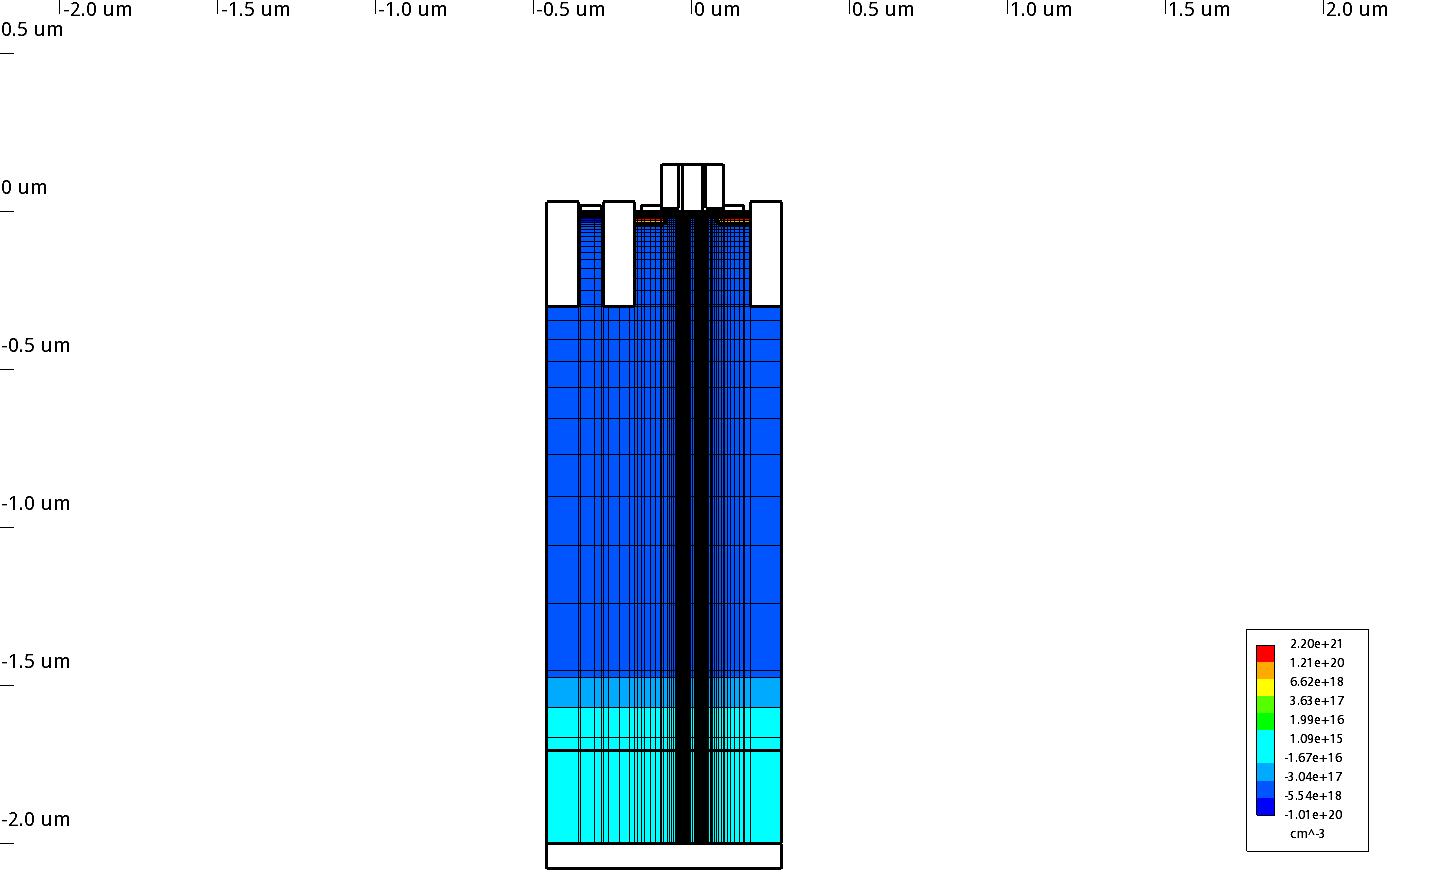
\includegraphics[width=0.7\textwidth]{image/01_device.png}
    \caption{任务1：器件结构示意图}
    \label{fig:t1_device}
\end{figure}

\begin{figure}[H]
    \centering
    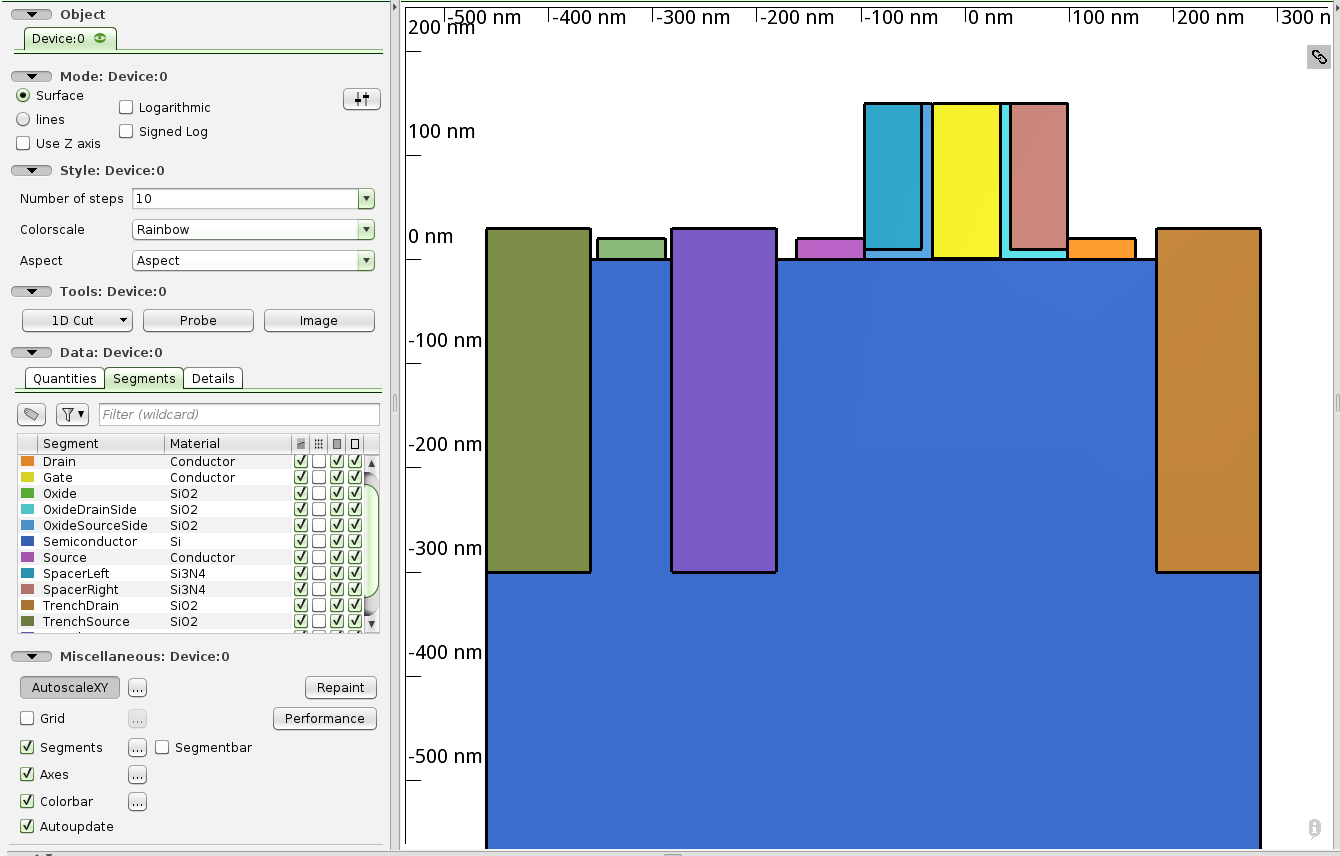
\includegraphics[width=0.7\textwidth]{image/01_device_part.png}
    \caption{任务1：器件结构图}
    \label{fig:t1_device_part}
\end{figure}

\begin{figure}[H]
    \centering
    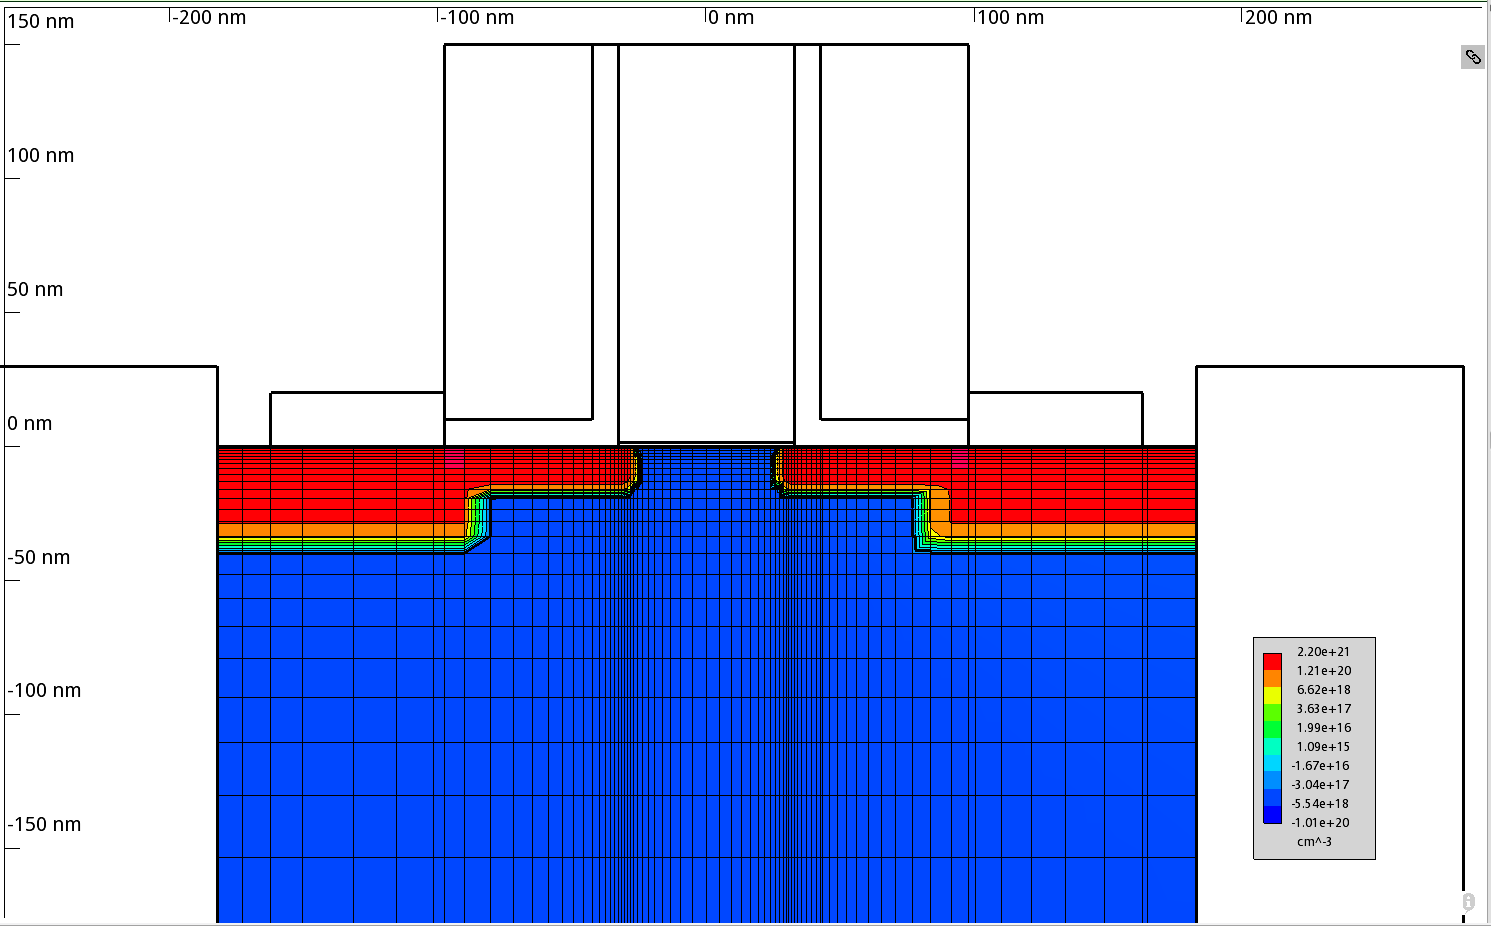
\includegraphics[width=0.7\textwidth]{image/01_device_doping.png}
    \caption{任务1：器件掺杂分布图}
    \label{fig:t1_device_doping}
\end{figure}
注：图2左侧两个 Trench 具有明确分工：靠内侧的第一个 Trench 紧邻工作源极，用于定义沟道起始边界，并抑制源端电子向衬底深处的无序扩散；靠外侧的第二个 Trench 用于“夹出”一块独立的 P-Well 区域，作为 Body Pick-up（衬底接头）布置位置。通过这两个 Trench 将工作源极电流路径与衬底接头路径在结构上分离，可在大电流工况下降低体区空穴堆积，从而抑制寄生双极效应触发，减小闩锁风险。

\subsubsection{IV 特性}

\begin{figure}[H]
    \centering
    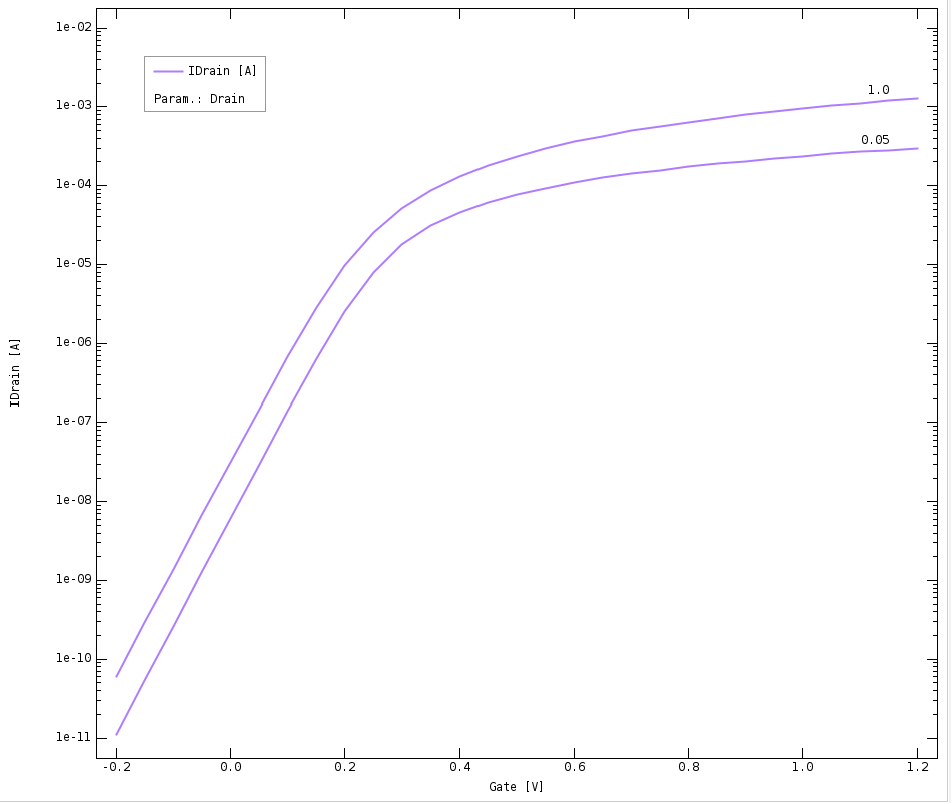
\includegraphics[width=0.7\textwidth]{image/01_IV.png}
    \caption{任务1：转移特性与输出特性结果图}
    \label{fig:t1_iv}
\end{figure}

从图~\ref{fig:t1_iv} 可见两条 $I_D$-$V_G$ 曲线均呈现典型 MOSFET 转移特性：低栅压区电流接近指数变化，中高栅压区逐步进入强反型导通。相同 $V_G$ 下，$V_{DS}=1\,\mathrm{V}$ 曲线始终高于 $V_{DS}=0.05\,\mathrm{V}$，说明高漏压增强了沟道电场并降低了有效势垒；在 $V_G\approx0.1\sim0.3\,\mathrm{V}$ 左右出现明显拐点，可作为阈值附近工作区的图形判据。

\subsubsection{1D Cut 验证}
\noindent\textbf{1) 电子浓度：}在低栅压偏置下，沟道中心出现明显“浓度谷”，处于弱反型/关断状态；当 $V_G$ 提升到约 $1.15\sim1.2\,\mathrm{V}$ 后，沟道中心浓度显著上升（相对低栅压抬升约 3 个数量级以上），表明连续反型通道已经形成（图~\ref{fig:t1_electron_concentration}）。

\begin{figure}[H]
    \centering
    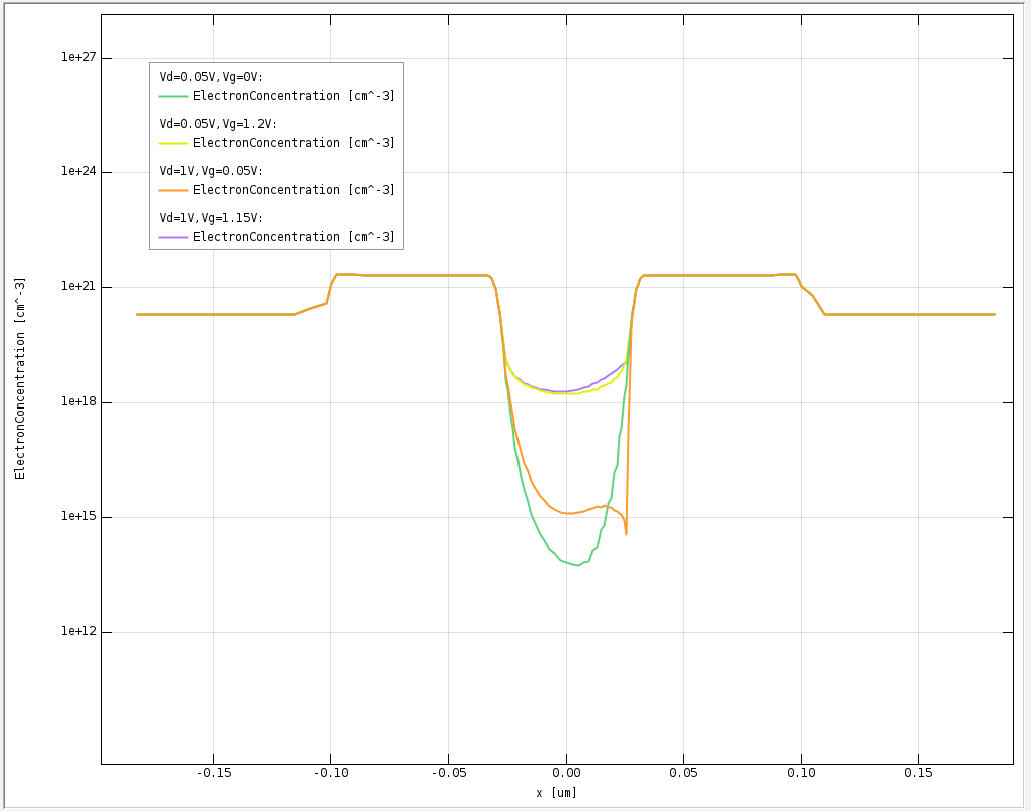
\includegraphics[width=0.7\textwidth]{image/01_ElectronConcentration.png}
    \caption{任务1：电子浓度分布（1D Cut）}
    \label{fig:t1_electron_concentration}
\end{figure}

\noindent\textbf{2) 电势：}在高 $V_{DS}$ 条件下漏端电势平台明显抬升，沟道最低势垒点上移并向源端传播，反映了漏端对沟道势垒调制作用，这与转移曲线上高漏压曲线整体上移相互一致；在 $V_{DS}$ 相同时，提高 $V_{GS}$ 会使沟道区域电势整体提高，降低沟道势垒并增强栅控，使器件更容易进入强反型导通（图~\ref{fig:t1_potential}）。

\begin{figure}[H]
    \centering
    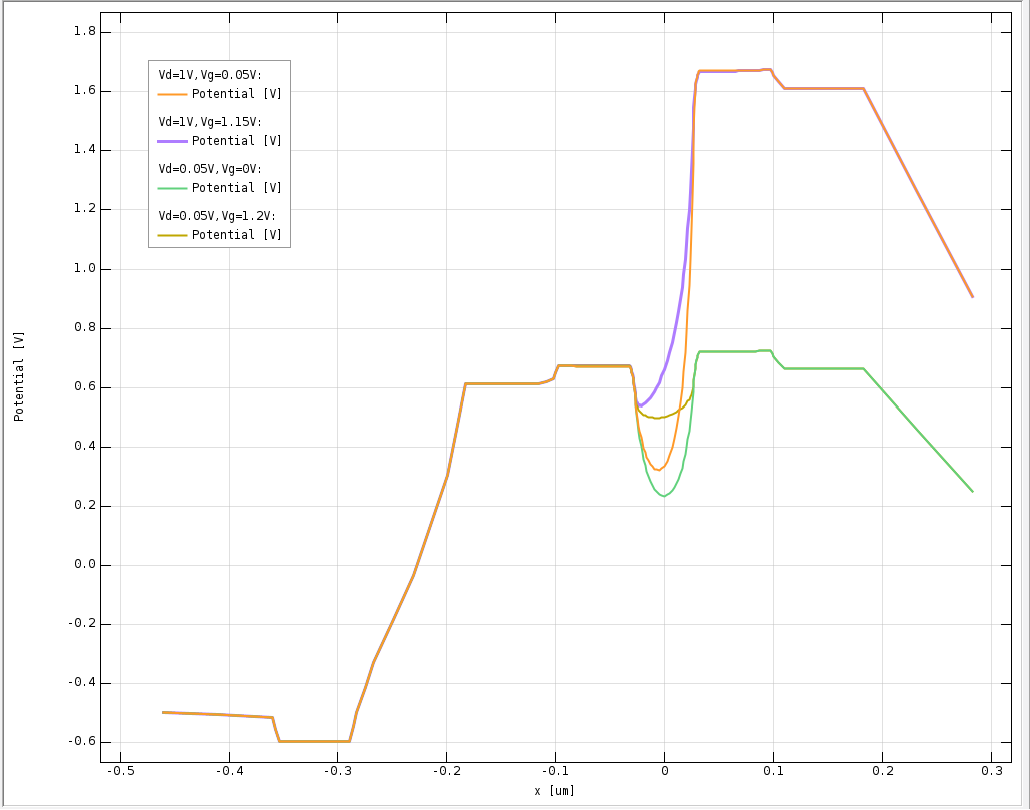
\includegraphics[width=0.7\textwidth]{image/01_Potential.png}
    \caption{任务1：电势分布（1D Cut）}
    \label{fig:t1_potential}
\end{figure}

\noindent\textbf{3) 能带：}提高 $V_{GS}$ 后沟道表面导带下移，源端注入势垒降低；同时高 $V_{DS}$ 下漏端能带倾斜更陡，表示更强横向电场与更高载流子漂移驱动，导通电流增加（图~\ref{fig:t1_bandenergy}）。

\begin{figure}[H]
    \centering
    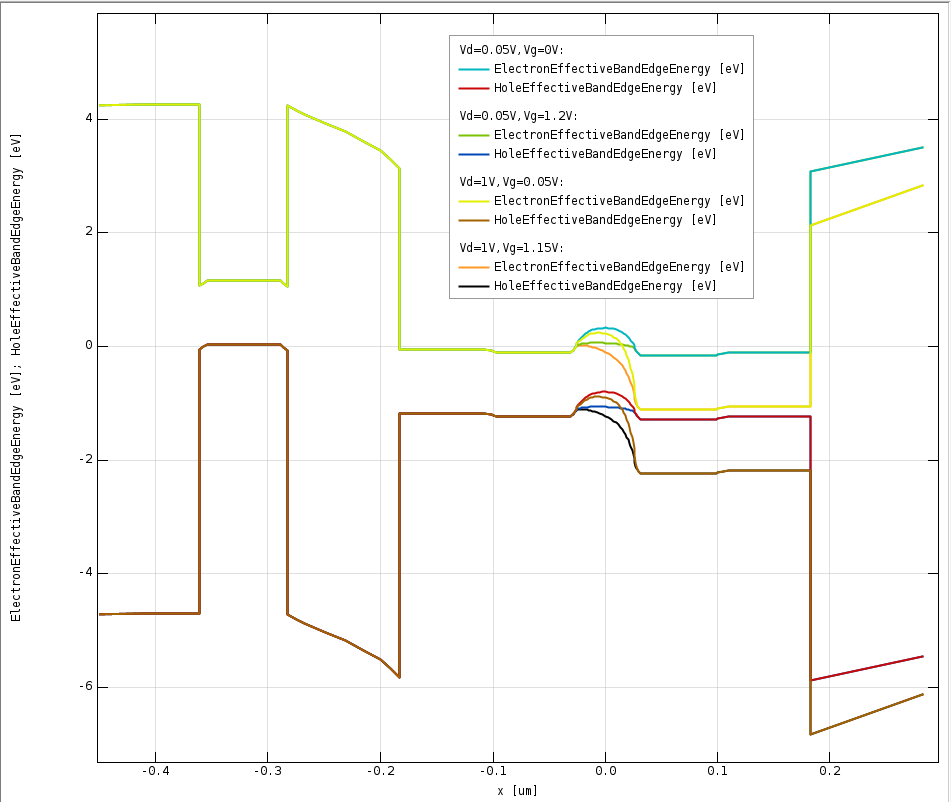
\includegraphics[width=0.7\textwidth]{image/01_bandenergy.png}
    \caption{任务1：能带分布（1D Cut）}
    \label{fig:t1_bandenergy}
\end{figure}


\subsubsection{归一化与参数提取结果}
归一化前后结果对比如图~\ref{fig:t1_normalization} 所示：归一化主要体现在关断到亚阈值区的横向平移，对齐了统一关断基准电流，可用于公平比较 $SS$、$I_{on}$、DIBL 等指标。

\begin{figure}[H]
    \centering
    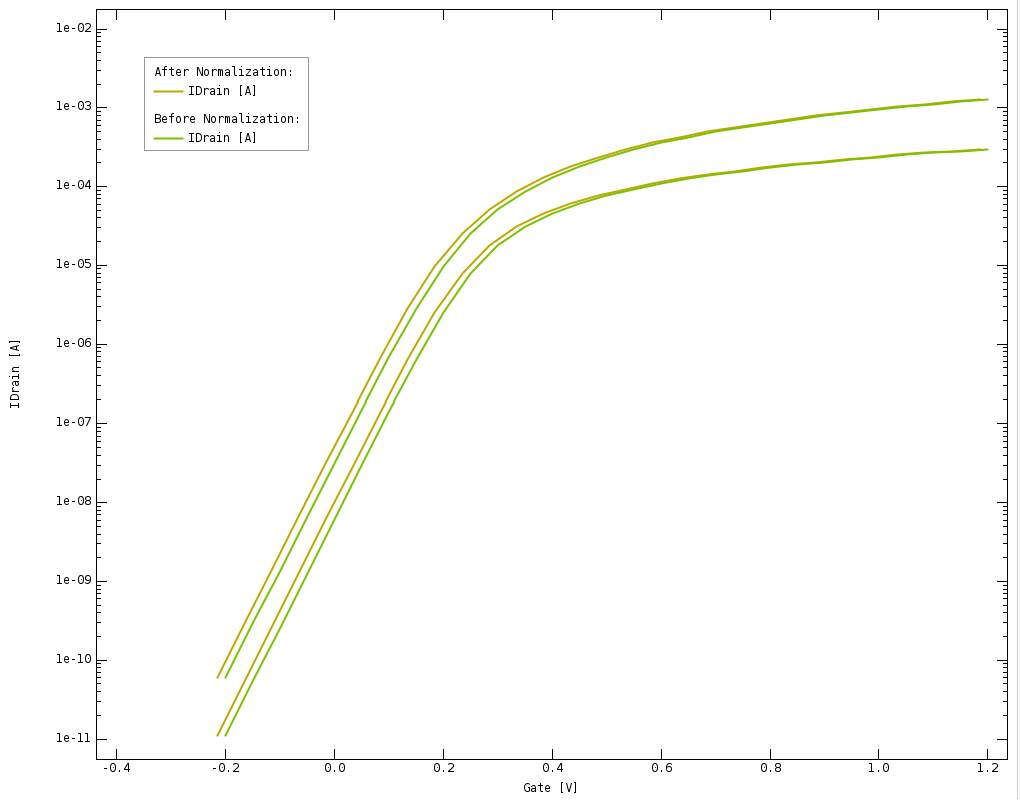
\includegraphics[width=0.7\textwidth]{image/01_normalization.png}
    \caption{任务1：电流归一化前后对比图}
    \label{fig:t1_normalization}
\end{figure}

进一步利用 Python 脚本提取关键指标参数，提取量包括：
\begin{itemize}
    \item $Vth\_lin$：线性区阈值电压（通常在低漏压，如 $V_{DS}=0.05\,\mathrm{V}$ 提取）。$Vth\_lin$ 升高可降低漏电但会抬高开启门限，可能牺牲导通电流。
    \item $Vth\_sat$：饱和区阈值电压（高漏压，如 $V_{DS}=1\,\mathrm{V}$ 提取）。与 $Vth\_lin$ 的差值反映漏端电场对势垒调制强弱。
    \item $Vg\_{gm\_max\_lin}$：线性区跨导峰值对应的栅压。该值越低通常表示较早进入高增益区，但需结合漏电与阈值综合判断。
    \item $gm\_max\_lin$：线性区最大跨导，表征低漏压下栅控效率；值越大说明单位栅压变化引起的电流增量越大。
    \item $Vg\_{gm\_max\_sat}$：饱和区跨导峰值对应栅压，反映高场工作点下达到最大增益所需的驱动栅压。
    \item $gm\_max\_sat$：饱和区最大跨导，体现高漏压条件下的栅控潜力；受速度饱和和迁移率退化影响更显著。
    \item $SS\_lin$：线性区亚阈值摆幅（mV/dec）。越小表示关断到导通过渡越陡，开关性能越好。
    \item $SS\_sat$：饱和区亚阈值摆幅。若显著大于 $SS\_lin$，通常提示漏端耦合增强与短沟道效应加重。
    \item $SS\_lin\_Vth$：在线性区以阈值附近窗口提取的亚阈值摆幅，用于评估阈值邻域的开关陡峭程度。
    \item $SS\_sat\_Vth$：在饱和区以阈值附近窗口提取的亚阈值摆幅，用于观察高漏压下阈值邻域的退化程度。
    \item $Ioff\_lin$：线性区关态漏电流。越小越有利于静态功耗控制与待机性能。
    \item $Ioff\_sat$：饱和区关态漏电流。该值偏大通常意味着 DIBL 或势垒降低问题更突出。
    \item $Ion\_sat$：饱和区开态电流，是数字驱动能力核心指标之一；越大通常有利于速度提升，但常与漏电控制存在权衡。
    \item $Ion\_lin$：线性区开态电流，反映低漏压导通能力与沟道电导特性。
    \item DIBL：漏致势垒降低，定义为高低漏压下阈值变化对漏压差的比值（mV/V）,越小表示短沟道效应更弱。
    \item $R\_on\_sat$：饱和偏置下等效导通电阻，反映高场工作时的导通损耗水平；越小越有利于大电流输出。
    \item $R\_on\_lin$：线性偏置下等效导通电阻，反映低场导通损耗与通道电阻特性；越小表示导通能力更强。
\end{itemize}

关键参数提取结果如图~\ref{fig:t1_parameter} 所示：其中 $Ioff\_lin=1.0\times10^{-8}\,\mathrm{A}$，验证了归一化后线性区关态电流对齐目标值的效果。

\begin{figure}[H]
    \centering
    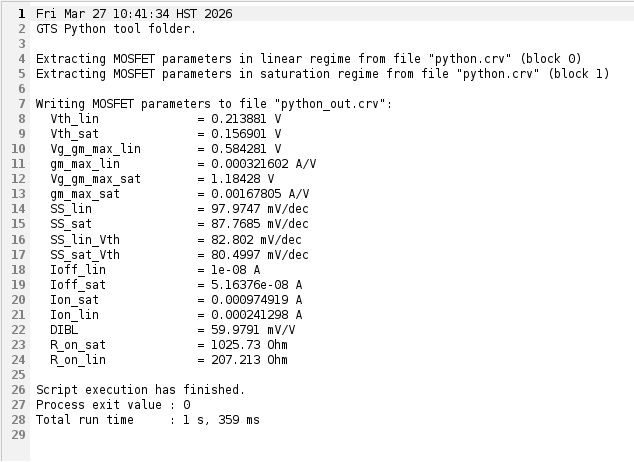
\includegraphics[width=0.9\textwidth]{image/01_parameter.png}
    \caption{任务1：关键参数提取结果图}
    \label{fig:t1_parameter}
\end{figure}

\section{任务 2：短沟道效应（SCE）分析}
\subsection{实验原理}
随着栅长（$L_g$）缩短，漏端对沟道电势的影响增强，导致栅极控制力下降。表现为阈值电压随栅长减小而下降（$V_{th}$ Roll-off）、亚阈值摆幅（SS）增大以及漏极诱导势垒降低（DIBL）。

定量上，阈值电压滚降可写为：
\begin{equation}
\Delta V_{th,roll\text{-}off}=V_{th}(L_{ref})-V_{th}(L_g)
\end{equation}
其中 $L_{ref}$ 取长沟道器件（100nm）作为基准。其物理原因在于：栅长减小时源/漏耗尽区的电势影响向沟道中部增强，沟道势垒被提前拉低，因此达到反型所需栅压降低，表现为 $V_{th}$ roll-off。

DIBL 常由高、低漏压下阈值电压差提取：
\begin{equation}
\mathrm{DIBL}=\frac{V_{th,lin}-V_{th,sat}}{V_{DS,sat}-V_{DS,lin}}\quad (\mathrm{mV/V})
\end{equation}
其中 $V_{th,lin}$ 与 $V_{th,sat}$ 分别对应线性区与饱和区偏置下提取的阈值电压。其物理机制是漏压升高后漏端电场增强，源端势垒被下拉，高漏压下更易导通，因此提取得到的阈值电压降低。栅长越短，漏端对沟道势垒调制越强，DIBL 通常越大。

亚阈值摆幅定义为：
\begin{equation}
SS=\left(\frac{d\log_{10}I_D}{dV_{GS}}\right)^{-1}
\end{equation}
其物理含义是栅压每改变一个数量级漏电流所需的电压增量。栅长减小时，漏端电场耦合增强，沟道势垒不再仅由栅极控制，亚阈值区对栅压调制效率下降，因此需要更大的 $V_{GS}$ 增量才能实现同样的电流数量级变化，表现为 $SS$ 增大（劣化）。

导通电流可近似写为
\begin{equation}
I_{on,long}\approx \frac{\mu_{eff}C_{ox}}{2}\frac{W}{L_g}(V_{GS}-V_{th})^2
\end{equation}
考虑短沟道速度饱和效应后，可写为
\begin{equation}
I_{on,SCE}\approx \frac{\mu_{eff}C_{ox}}{2}\frac{W}{L_g}\frac{(V_{GS}-V_{th})^2}{1+\dfrac{V_{GS}-V_{th}}{E_{sat}L_g}}
\end{equation}
其中 $E_{sat}$ 为速度饱和相关临界场。在长沟道体制下，$I_{on}\propto W/L_g$，缩小 $L_g$ 能有效提升电流。但在短沟道下，当 $\dfrac{V_{GS}-V_{th}}{E_{sat}L_g}\gg 1$ 时，分母由速度饱和项主导，此时 $I_{on}$ 趋向于 $\propto W \cdot E_{sat} \cdot (V_{GS}-V_{th})$，与 $L_g$ 的关联被打破。进一步叠加迁移率退化与其他短沟道效应，$I_{on}$ 随 $L_g$ 继续缩短而改善的优势消失，最终导致指标恶化。

\subsection{预期结果}
\subsubsection{IV 曲线对比}
IV 曲线对比可直接看出三点：第一，在低栅压区（约 $V_G<0.1\,\mathrm{V}$），大$V_d$下45nm 曲线明显高于 65nm 与 100nm，说明短沟道器件关态泄漏更高；第二，在阈值附近（约 $0.1\sim0.3\,\mathrm{V}$），45nm 曲线在不同$V_d$下曲线差异更大，反映漏端电场耦合对沟道势垒调制更强；第三，在高栅压区，两组偏置（图中标注 1.0 与 0.05）下三者电流差距收敛，45nm/65nm 曲线略高于 100nm，表明缩短栅长主要带来低压区泄漏抬升，而高栅压驱动提升并不成比例。

不同栅长器件的 IV 曲线对比如图~\ref{fig:t2_iv} 所示。

\begin{figure}[H]
    \centering
    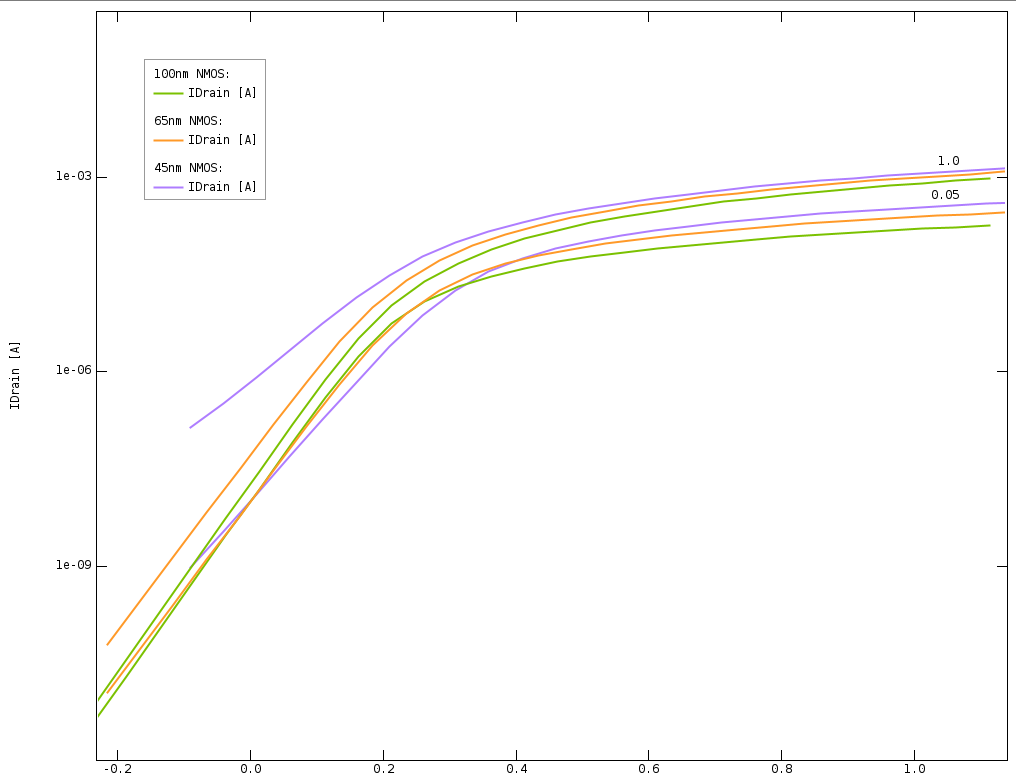
\includegraphics[width=0.7\textwidth]{image/02_IV.png}
    \caption{任务2：不同栅长器件 IV 曲线对比}
    \label{fig:t2_iv}
\end{figure}

\subsubsection{\texorpdfstring{$SS$、$I_{on}$ 与 $DIBL$ 对比}{SS、Ion 与 DIBL 对比}}
由图~\ref{fig:t2_iv} 与图~\ref{fig:t2_ss_ion_dibl} 可形成一致结论：在低栅压区，45nm 曲线在不同$V_d$下明显上抬，对应 DIBL 从 100nm 的 $29.11\,\mathrm{mV/V}$ 升至 45nm 的 $145.62\,\mathrm{mV/V}$；同时其亚阈值段更平缓，对应 $SS_{sat}$ 由 88.66/87.77 mV/dec（100nm/65nm）恶化到 121.27 mV/dec（45nm）。在高栅压区，三者导通电流排序为 45nm $>$ 65nm $>$ 100nm，对应 $I_{on,sat}$ 分别约为 $1.11\times10^{-3}$、$9.75\times10^{-4}$、$7.89\times10^{-4}\,\mathrm{A}$。这说明三参数对比的核心特征是：45nm 虽具有更高 $I_{on}$，但同时出现“DIBL 显著增大 + SS 劣化”，需要在驱动能力与短沟道控制之间进行权衡。

\begin{figure}[H]
    \centering
    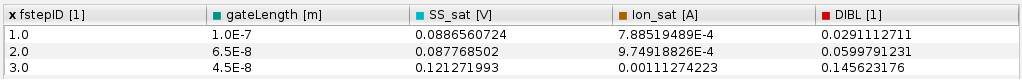
\includegraphics[width=0.9\textwidth]{image/02_SS_Ion_DIBL.png}
    \caption{任务2：SS、$I_{on}$ 与 DIBL 指标对比}
    \label{fig:t2_ss_ion_dibl}
\end{figure}

\subsubsection{\texorpdfstring{阈值滚降（$V_{th}$ roll-off）}{阈值滚降（Vth roll-off）}}
实验结果显示，随着 $L_g$ 缩短，$V_{th}$ 出现明显 roll-off：由 100nm 的 $0.269\,\mathrm{V}$ 降至 65nm 的 $0.173\,\mathrm{V}$，在 45nm 进一步降至约 $-5.7\,\mathrm{mV}$，短沟道势垒控制显著削弱。

对应的阈值滚降（roll-off）结果如图~\ref{fig:t2_vth} 所示。

\begin{figure}[H]
    \centering
    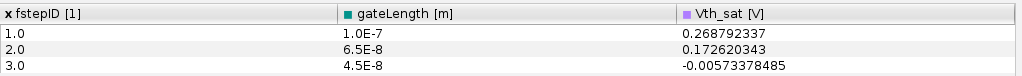
\includegraphics[width=0.9\textwidth]{image/02_Vth.png}
    \caption{任务2：阈值电压 roll-off 对比}
    \label{fig:t2_vth}
\end{figure}

\section{任务 3：45nm 平面 NMOS 的优化设计}
\subsection{实验原理}
\textbf{(1) $SS$ 优化：}
亚阈值摆幅满足
\begin{equation}
SS\approx (\ln 10)\frac{kT}{q}\left(1+\frac{C_{dep}}{C_{ox}}\right),\qquad C_{ox}=\frac{\varepsilon_{ox}}{T_{ox}}
\end{equation}
减小 $T_{ox}$ 可增大 $C_{ox}$ 并降低 $C_{dep}/C_{ox}$，从而压低 $SS$。

\textbf{(2) $I_{on}$ 优化：}
导通电流近似为
\begin{equation}
I_{on}\approx \frac{1}{2}\mu_{eff}C_{ox}\frac{W}{L}(V_{GS}-V_{th})^2
\end{equation}
减小 $T_{ox}$ 提升 $C_{ox}$ 可提高 $I_{on}$。

\textbf{(3) DIBL 优化：}
DIBL 反映高低漏压下阈值偏移，实质是漏端电场对沟道势垒的耦合强弱。减小 $T_{ox}$ 可增强栅极主导控制；提高沟道/井区有效掺杂可提高势垒刚性、降低电荷共享效应，从而减小 DIBL。

\textbf{(4) $V_{th}$ roll-off 优化：}
阈值滚降定义为
\begin{equation}
\Delta V_{th,roll\text{-}off}=V_{th}(L_{ref})-V_{th}(45\,\mathrm{nm})
\end{equation}
且
\begin{equation}
V_{th}=V_{fb}+2\phi_F+\frac{\sqrt{4\varepsilon_{si}qN_A\phi_F}}{C_{ox}}
\end{equation}
说明 $T_{ox}$ 与掺杂共同决定阈值稳定性。优化时需通过“较薄栅氧 + 适度增掺”抑制 45nm 器件阈值下滑，同时避免因过度增掺带来 $I_{on}$ 损失。

\subsection{设计要求与约束}
\begin{itemize}
    \item 指标：$SS < 90$ mV/dec, $I_{on} > 9.5 \times 10^{-4}$ A/um, $DIBL < 90$ mV/V。
    \item 同时要求：相对 100nm 基准的饱和态阈值滚降满足 $V_{th}$ Roll-off $< 180$ mV。
    \item 约束：$T_{ox}$ 需在 $[0.8, 2]$ nm 区间内，仅限调整栅氧和掺杂。
\end{itemize}

\subsection{仿真与分析}
针对 45nm 初始器件（$SS\approx121.27\,\mathrm{mV/dec}$、$I_{on,sat}\approx1.11\times10^{-3}\,\mathrm{A}$、DIBL$\approx145.62\,\mathrm{mV/V}$）不达标的问题，采用 DOE 对 $T_{ox}$ 与沟道掺杂进行联合优化。

优化结果显示，较优参数点位于 $T_{ox}=1.0\,\mathrm{nm}$、dopingWell$=6.0\times10^{18}\,\mathrm{cm^{-3}}$。在该点，$V_{th,sat}\approx0.319\,\mathrm{V}$（对应 $\Delta V_{th,roll\text{-}off}=0.269-0.319=-0.050\,\mathrm{V}$），$SS_{sat}\approx84.46\,\mathrm{mV/dec}$，$I_{on,sat}\approx1.42\times10^{-3}\,\mathrm{A}$，DIBL$\approx52.80\,\mathrm{mV/V}$，四项核心指标均满足设计约束。

\begin{figure}[H]
    \centering
    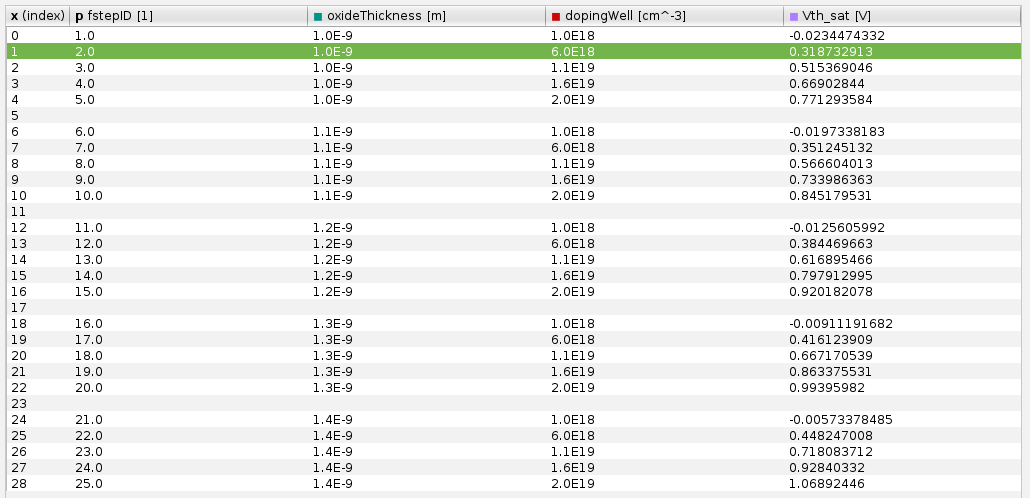
\includegraphics[width=0.9\textwidth]{image/03_Vth_Optimization.png}
    \caption{任务3：优化前后阈值相关指标对比}
    \label{fig:t3_vth_optimization}
\end{figure}

\begin{figure}[H]
    \centering
    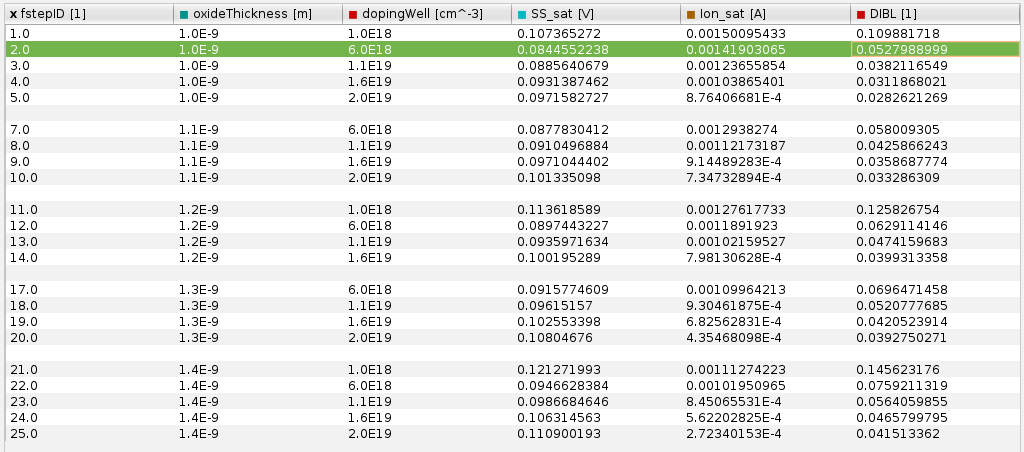
\includegraphics[width=0.9\textwidth]{image/03_SS_Ion_DIBL_Optimization.png}
    \caption{任务3：优化前后 SS、$I_{on}$ 与 DIBL 指标对比}
    \label{fig:t3_ss_ion_dibl_optimization}
\end{figure}


\end{document}